\documentclass[a4paper,10pt]{article}
\usepackage[utf8]{inputenc}
\usepackage{graphicx}
\usepackage[thinlines]{easytable}
\usepackage{enumitem}
\usepackage{amsmath}
\usepackage{bbm}
\usepackage{amsfonts}
\usepackage{listings}
\usepackage{pbox}
\usepackage[usenames,dvipsnames]{color}
 
% This is the color used for MATLAB comments below
\definecolor{MyDarkGreen}{rgb}{0.0,0.4,0.0}
 
% For faster processing, load Matlab syntax for listings
\lstloadlanguages{Matlab}%
\lstset{language=Matlab, % Use MATLAB
frame=single, % Single frame around code
basicstyle=\tiny\ttfamily, % Use small true type font
keywordstyle=[1]\color{Blue}\bfseries, % MATLAB functions bold and blue
keywordstyle=[2]\color{Purple}, % MATLAB function arguments purple
keywordstyle=[3]\color{Blue}\underbar, % User functions underlined and blue
identifierstyle=, % Nothing special about identifiers
% Comments small dark green courier
commentstyle=\usefont{T1}{pcr}{m}{sl}\color{MyDarkGreen}\small,
stringstyle=\color{Purple}, % Strings are purple
showstringspaces=false, % Don't put marks in string spaces
tabsize=5, % 5 spaces per tab
%
%%% Put standard MATLAB functions not included in the default
%%% language here
morekeywords={xlim,ylim,var,alpha,factorial,poissrnd,normpdf,normcdf},
%
%%% Put MATLAB function parameters here
morekeywords=[2]{on, off, interp},
%
%%% Put user defined functions here
morekeywords=[3]{FindESS, homework_example},
%
morecomment=[l][\color{Blue}]{...}, % Line continuation (...) like blue comment
numbers=left, % Line numbers on left
firstnumber=1, % Line numbers start with line 1
numberstyle=\tiny\color{Blue}, % Line numbers are blue
stepnumber=5 % Line numbers go in steps of 5
}
\newcommand\scalemath[2]{\scalebox{#1}{\mbox{\ensuremath{\displaystyle #2}}}}



%opening
\title{Equations Of Motion Of a Wheeled Inverted Pendulum}
\author{Munzir Zafar}

\begin{document}

\maketitle

In an earlier report \cite{munzir2013balancing} we had derived using Newton-Euler method the equations of
motion of a wheeled inverted pendulum. But this model did not take into account the spin motion of the
robot. Before attempting to derive the new equations including the spin, we will look at the equations
derived in the existing literature.

\section{Using the equation from \cite{kim2005dynamic}}

The equations derived in \cite{kim2005dynamic} for the motion of two-wheeled inverted pendulum robot are:
\begin{align}
 &3(m_c+m_s)\ddot{x}-m_sdcos\phi\ddot{\phi}+m_sdsin\phi({\dot{\phi}}^2+{\dot{\psi}}^2)=-\frac{\alpha_3+\beta_3}{R} \label{eq1}\\
 &\left\lbrace(3L^2+1/2R^2)m_c+m_sd^2sin^2\phi+I_2\right\rbrace\ddot{\psi}+m_sd^2sin\phi cos\phi\dot{\psi}\dot{\phi}=\frac{L}{R}(\alpha_3-\beta_3) \label{eq2}\\
 &m_sdcos\phi\ddot{x}+(-m_sd^2-I_3)\ddot{\phi}+m_sd^2sin\phi cos\phi {\dot{\phi}}^2+m_sgdsin\phi=\alpha_3+\beta_3 \label{eq3}
\end{align} where,

$\dot{x}$ is the heading speed of the robot 

$\phi$ is the rotation of the C.G. about $n_3$-directional 

$\psi$ is the heading angle (angle between $n_1$ and the world frame) 

$\alpha_3$ is the torque of the left wheel 

$\beta_3$ is the torque of the right wheel 

$m_c$ is the mass of the wheel 

$m_s$ is the mass of the body 

$d$ is the distance between wheel axis to C.G. 

$R$ is the radius of the wheel 

$L$ is the half distance between wheels 

$I_2$ is the $n_2$-directional rotational inertia of the body 

$I_3$ is the $n_3$-directional rotational inertia of the body 

$n_2$ is the unit vector pointing vertically upwards 

$n_3$ is the unit vector pointing from the left wheel to the right wheel \newline

The equations that we had derived in our earlier report \cite{munzir2013balancing} did not include
the rotation about the vertical axis of the robot. One of the equations above represent that motion.
We will try to first match the equations we had derived with the equations listed above as a sanity
check. Then we will write down the thrid equation using the variables that we had used in our 
earlier report. Then we will attempt to derive the equation using Newton-Euler method. Equations from
our earlier report are listed here:

\begin{align}
 &[(m+M)r+I_w/r+\eta^2I_m/r]\ddot{x}+(mrlcos\theta-\eta^2I_m)\ddot{\theta} = K_fu-\tau_f+F_{ext}rcos\theta+mrl\dot{\theta}^2sin\theta \label{eq4}\\
 &(mlcos\theta - \eta^2I_m/r)\ddot{x} + (ml^2 + I + \eta^2I_m)\ddot{\theta} = - K_fu + \tau_f + F_{ext}l + mglsin\theta \label{eq5}
\end{align} where,

$m$ is the mass of the body

$M$ is the mass of the wheels

$r$ is the radius of the wheel

$I_w$ is the inertia of the wheel

$\eta$ is the gear ratio of the motor

$I_m$ is the motor inertia

$\dot{x}$ is the heading speed

$l$ is the distance between wheel axis and the C.G.

$\theta$ is the rotation of the C.G. about the wheel axis

$K_f$ is the torque to current ratio of the motor

$\tau_f$ is the frictional torque on the wheels

$F_{ext}$ is the external force being applied at the C.G. perpendicular to $l$

$I$ is the inertia of the robot about the wheel axis \newline

Using the symbols used in equations \ref{eq4}-\ref{eq5}, we re-write the equations \ref{eq1}-\ref{eq3}:
\begin{align}
 &3(M+m)\ddot{x}-mlcos\theta\ddot{\theta}+mlsin\theta({\dot{\theta}}^2+{\dot{\psi}}^2)=-\frac{K_f(u_1+u_2)}{r} \label{eq6} \\
 &\left\lbrace(3L^2+1/2r^2)M+ml^2sin^2\theta+I_2\right\rbrace\ddot{\psi}+ml^2sin\theta cos\theta\dot{\psi}\dot{\theta}=\frac{L}{r}K_f(u_1-u_2) \label{eq7} \\
 &mlcos\theta\ddot{x}+(-ml^2-I)\ddot{\theta}+ml^2sin\theta cos\theta {\dot{\theta}}^2+mglsin\theta=K_f(u_1+u_2) \label{eq8}
\end{align} where, we have retained the symbols for quantities that do not appear in equations 
\ref{eq4}-\ref{eq5} i.e. $\psi$ and $I_2$ which represent the heading direction and the inertia 
about the vertical axis respectively.

In equations \ref{eq6}-\ref{eq8}, we make the following observations:
\begin{enumerate}[label=(\roman*)]
 \item Equations \ref{eq6} and \ref{eq8} are the equivalents of the equations \ref{eq4} and \ref{eq5} respectively
 \item The equations \ref{eq6} and \ref{eq8} ignore the effects of wheel inertia $I_w$, the motor inertia $I_m$, frictional
 torque $\tau_f$ at the wheel motor and the external force $F_{ext}$, all of which were considered in equations \ref{eq4} and \ref{eq5}
 \item The terms containing $\ddot{x}$ in equations \ref{eq4} and \ref{eq5} appear with opposite signs in equations \ref{eq6} and \ref{eq8} \label{item:ddotx}
 \item The term $mrlsin\theta{\dot\theta}^2$ of equation \ref{eq4} appears as $mrlsin\theta({\dot\theta}^2+{\dot\psi}^2)$ in equation \ref{eq6} \label{item:psi}
 \item Equation \ref{eq4} does not contain the coefficient $3$ with the $\ddot{x}$ term which appears in equation \ref{eq6} \label{item:coeff3}
 \item Equation \ref{eq5} does not contain the term $ml^2sin\theta cos\theta {\dot{\theta}}^2$ which appears in equation \ref{eq8} \label{item:corriolis}
\end{enumerate}

 Point number \ref{item:ddotx} may be explained by assuming that the two derivations assumed $x$ increases in different directions.
Point number \ref{item:psi} may be explained by the fact that equations \ref{eq4} and \ref{eq5} assume constant heading direction i.e. $\dot\psi=0$
But the last two points are not easy to explain. An interesting fact regarding point regarding \ref{item:coeff3} is that the paper \cite{kim2005dynamic}
changes the term from $3(m_c+m_s)$ in the original equation that we cited aboce to $3m_c+m_s$ in the later equations of the same paper. It appears that
the latter expression is more accurate and basically $3m_c$ represents the mass of three wheels of equal mass, one of which is a supporting wheel.
The paper discusses supporting wheels at length, so it won't be surprise. That solves the mystery of the second last point. What remains now is to
discuss the very last point. Since we see that there is a typo done in the earlier equation, we can expect this term to have a typo, in that it
is missing a $\dot\psi$ term. If this was true we will safely assume that the reason this term isn't present in our earlier analysis (i.e. equations 
\ref{eq4} and \ref{eq5}) is because we assumed constant heading direction i.e. $\dot{\psi}=0$.

\section{Using equations from \cite{li2012advanced}}
In the book \cite{li2012advanced} following equations of motion are derived:

\begin{align}
 &\left(M+2M_w+m+2\frac{I_w}{r^2}\right)\dot{v}+ml\ddot{\alpha}cos\alpha-ml{\dot{\alpha}}^2sin\alpha = \frac{\tau_l}{r}+\frac{\tau_r}{r}+d_l+d_r \label{eq9} \\
 &\left(I_p+2\left(M_w+\frac{I_w}{r^2}\right)d^2\right)\dot{\omega}=2d\left(\frac{\tau_l}{r}-\frac{\tau_r}{r}+d_l-d_r\right) \label{eq10} \\
 &ml\dot{v}cos\alpha+\left(ml^2+I_M\right)\ddot{\alpha}-mglsin\alpha=0 \label{eq11}
\end{align} where,

$M$ is the mass of the platform

$M_w$ is the mass of one wheel	

$m$ is the mass of the robot

$I_w$ is the inertia of one wheel

$r$ is the radius of one wheel

$v$ is the heading speed of the wheel

$l$ is the distance from C.G. to wheel axis

$\alpha$ is the rotation of C.G. about the wheel axis

$\tau_l$ is the torque applied by left wheel motor

$\tau_r$ is the torque applied by right wheem motor

$d_l$ is the external force acting on the left wheel

$d_r$ is the external force acting on the right wheel
\newline
Now, replacing these variables with the ones we had used in \cite{munzir2013balancing}, 
equations, \ref{eq9}-\ref{eq11} become:

\begin{align}
 &\left(M_p+M+m+\frac{I_w}{r^2}\right)\ddot{x}+ml\ddot{\theta}cos\theta-ml{\dot{\theta}}^2sin\theta = \frac{K_fu_1}{r}+\frac{K_fu_2}{r}+d_l+d_r \label{eq12} \\
 &\left(I_z+\left(M+\frac{I_w}{r^2}\right)L^2\right)\ddot{\psi}=2L\left(\frac{K_fu_1}{r}-\frac{K_fu_2}{r}+d_l-d_r\right) \label{eq13} \\
 &ml\ddot{x}cos\theta+\left(ml^2+I\right)\ddot{\theta}-mglsin\theta=0 \label{eq14}
\end{align}

Following observation are made:
\begin{enumerate}[label=(\roman*)]
 \item Equations \ref{eq12} and \ref{eq14} are the equivalents of equations \ref{eq4} and \ref{eq5} respectively
 \item Equation \ref{eq13} represents spin
 \item There is no difference between equation \ref{eq12} and \ref{eq4} except that $(a)$ equation \ref{eq4} considers
 motor inertia $I_m$ while \ref{eq12} does not and $(b)$ eq \ref{eq12} consider platform as different from the pendulum while 
 krang has no such thing as a platform so the additional mass term $M_p$ in equation \ref{eq12} is not there in \ref{eq4}
 \item There is no difference between equation \ref{eq12} and \ref{eq4} except that $(a)$ equation \ref{eq4} considers
 motor inertia $I_m$ while \ref{eq12} does not and $(b)$ the effect of counter torque on the pendulum is not considered
 in the eq \ref{eq12} as the pendulum does not experience the countertorque due to it being on a platform and not 
 directly attached to the motor so we don't see any term on the right hand side of eq \ref{eq12}
 \item Equation \ref{eq13} when compared with eq \ref{eq7} that represented spin in the previous section we see that
 the coefficient of $\ddot{\psi}$ was a funtion of $\theta$ there but here it is not. The reason is that $I_z$ term
 in eq \ref{eq13} is actually a function of $\theta$. That function is written over there but not here.
 \item Also there is a $\dot{\psi}$ term in equation \ref{eq7} that is not there in eq \ref{eq13}. It seems like equation \ref{eq7}
 makes more sense as a non-zero $\dot{\theta}$ will introduce a corriolis force in the system that is apparently not taken into
 account by equation \ref{eq13}
\end{enumerate}

\section{Comparing \cite{kim2005dynamic} and \cite{li2012advanced}}

It appears that the analysis done by \cite{kim2005dynamic} is more correct with regards to understanding of the dynamics,
only that it seems to have introduced some typos and thus can't be trusted blindly. The analysis in \cite{li2012advanced}
on the other hand is very cleanly explained and does not contain typos, it is weak in representation of all dynamic effects
in the system. The way we will move forward is by using the expressions for velocities that are more completely derived
in \cite{kim2005dynamic} and use the detailed procedures explained in \cite{li2012advanced} to come up with expressions
of dynamics that are useful for our purposes.


\section{Deriving the Dynamic Model for our robot}



\begin{figure}
 \centering
 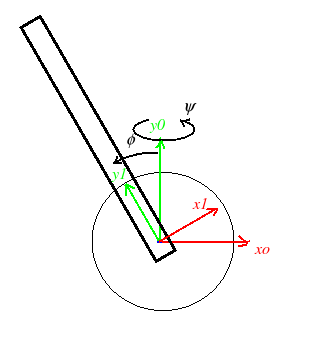
\includegraphics[width=0.3\textwidth]{Figures/referenceImage.png}
 \caption{Frames of references on the robot}
 \label{fig:frames}
\end{figure}

\subsection{Kinetic and Potential Energy of the Body}
\begin{align} \begin{split}
 {}^0V_0 &= \left[\begin{matrix} \dot{x} & 0 & 0 \end{matrix}\right]^T \\
 {}^0\omega_0 &= \left[\begin{matrix} 0 & \dot{\psi} & 0 \end{matrix}\right]^T \\
 {}^0\mathbf{g} &= \left[\begin{matrix} 0 & -g & 0 \end{matrix}\right]^T \\
 {}^0T_1 &= \left[\begin{matrix}  & {}^0A_1 & & {}^0P_1 \\ 0 & 0 & 0 & 1\end{matrix}\right]
 = \left[\begin{matrix} {}^0\mathbf{x}_1 & {}^0\mathbf{y}_1 & {}0^\mathbf{z}_1 & {}^0P_1 \\ 0 & 0 & 0 & 1\end{matrix}\right] 
 = \left[\begin{matrix} cos\phi & -sin\phi & 0 & 0 \\ sin\phi & cos\phi & 0 & 0 \\ 0 & 0 & 1 & 0 \\ 0 & 0 & 0 & 1\end{matrix}\right] \\
 {}^1e_1 &= \left[\begin{matrix} 0 & 0 & 1 \end{matrix}\right]^T \\
 \dot{q}_1 &= \dot{\phi} \\
\end{split} \end{align}

\begin{align} \begin{split}
 {}^1\omega_1 &= {}^1A_0{}^0\omega_0+{}^1e_1\dot{q}_1 \\
 {}^1V_1 &= {}^1A_0{}^0\left({}^0V_0+{}^0\omega_0\times {}^0P_1\right) \\
\end{split} \end{align}

\begin{align} \begin{split}
 E_1 &= \frac{1}{2}\left(\omega_1^TJ_{G1}\omega_1+M_1V_1^TV_1+2\mathbf{MS}_1^T(V_1\times\omega_1)\right) \\
 U_1 &= -\left[\begin{matrix}{}^0\mathbf{g}^T & 0 \end{matrix} \right]{}^0T_1\left[\begin{matrix}\mathbf{MS}_1 \\ M_1 \end{matrix} \right]
\end{split}\end{align}

\subsection{Kinetic and Potential Energy of the Wheels}
\begin{align} \begin{split}
 {}^L\omega_L &= \left[\begin{matrix} 0 & \dot{\psi} & -\frac{1}{R}\dot{x}+\frac{L}{2R}\dot{\psi} \end{matrix}\right]^T \\
 {}^LV_L &= \left[\begin{matrix} \dot{x}-\dot{\psi}\frac{L}{2} & 0 & 0 \end{matrix}\right]^T \\
 E_L &= \frac{1}{2}\left(\omega_L^TJ_{Gw}\omega_L+M_wV_L^TV_L+2\mathbf{MS}_w^T(V_L\times\omega_L)\right) 
\end{split}\end{align}
\begin{align} \begin{split}
 {}^R\omega_R &= \left[\begin{matrix} 0 & \dot{\psi} & -\frac{1}{R}\dot{x}-\frac{L}{2R}\dot{\psi} \end{matrix}\right]^T \\
 {}^RV_R &= \left[\begin{matrix} \dot{x}+\dot{\psi}\frac{L}{2} & 0 & 0 \end{matrix}\right]^T \\
 E_R &= \frac{1}{2}\left(\omega_R^TJ_{Gw}\omega_R+M_wV_R^TV_R+2\mathbf{MS}_w^T(V_R\times\omega_R)\right) 
\end{split}\end{align}

\subsection{Applying Lagrange Method to find matrices $\mathbf{A}$, $\mathbf{C}$ and $\mathbf{Q}$}
The Lagrange formulation describes the behavior of a dynamic system in terms of work and energy stored in the
system. The Lagrange equations are commonly written in the form:
\begin{align}
  \Gamma_i = \frac{d}{dt}\frac{\partial L}{\partial \dot{q}_i}-\frac{\partial L}{\partial q_i} \quad for\; i \in \mathbb{F} \label{eq:Lagrange}
\end{align} where $L$ is the Lagrangian of the robot defined as the difference berween the kinetic energy $E$ and potential 
energy $U$ of the system:
\[
 L = E-U
\]
\subsubsection{General Form of the Dynamic Equations}
The kinetic energy of the system is a quadratic function in the joint velocities such that:
\begin{align}
 &E = \frac{1}{2}\mathbf{\dot{q}^TA\dot{q}}
\end{align} where $\mathbf{A}$ is the $n\times n$ symmetric and positive definite \textit{inertia matrix} of the robot.
Its elements are functions of the joint positions. The $(i,j)$ element of $\mathbf{A}$ is denoted $A_{ij}$. Since the 
potential energy is a function of the joint positions, equation \ref{eq:Lagrange} leads to:
\begin{align}
 &\mathbf{\Gamma=A(q)\ddot{q}+C(q,\dot{q})\dot{q}+Q(q)}
\end{align} where:
\begin{itemize}
 \item $\mathbf{C(q,\dot{q})\dot{q}}$ is the $n\times 1$ vector of Coriolis and centrifugal torques, such that: 
 $\mathbf{C\dot{q} = \dot{A}\dot{q}}-\frac{\partial E}{\partial \mathbf{q}}$
 \item $\mathbf{Q} = \left[\begin{matrix} Q_1 & Q_2 & Q_3 & Q_{4l} & ... & Q_{10l} & Q_{4r} & ... & Q_{10r} \end{matrix} \right]^T$ 
 is the vector of gravity torques
\end{itemize}
So the dynamic model of a tree-structured robot is described by $n$ coupled and nonlinear second order differential
equations. The elements of $\mathbf{A}$, $\mathbf{C}$ and $\mathbf{Q}$ are functions of geometric and inertial 
parameters of the robot.

\subsubsection{Computation of the elements of $\mathbf{A}$, $\mathbf{C}$ and $\mathbf{Q}$}
To compute the elements of $\mathbf{A}$, $\mathbf{C}$ and $\mathbf{Q}$, we begin by symbollically computing the 
expressions of the kinetic and potential energies of all the links of the robot. Then we proceed as follows:
\begin{itemize}
  \item the elements $A_{ij}$ is equal to the coefficient of $\left(\frac{\dot{q}_i^2}{2}\right)$ in the expression of
  the kinetic energy, while $A_{ij}$, for $i \neq j$, is equal to the coefficient of $\dot{q}_i\dot{q}_j$
  \item for calculating the elements of $\mathbf{C}$, there exist several forms of the vector $\mathbf{C(q,\dot{q})\dot{q}}$.
 Using the \textit{Christoffell symbols} $c_{i,jk}$, the $(i,j)$ elements of the matrix $\mathbf{C}$ can be written as:
 \begin{align}
  \begin{cases}
   C_{ij} = \sum\limits^{n}_{k=1}c_{i,jk}\dot{q}_k \\
   c_{i,jk} = \frac{1}{2}\left[\frac{\partial A_{ij}}{\partial q_k} + \frac{\partial A_{ik}}{\partial q_j} - \frac{\partial A_{jk}}{\partial q_i}\right]
  \end{cases} \label{eqC}
 \end{align}
 \item The $Q_i$ element of the vector $\mathbf{Q}$ is calculated according to:
 \begin{align}
  Q_i = \frac{\partial U}{\partial q_i}
 \end{align}
\end{itemize}

\subsubsection{Resulting Matrices}
\begin{align} \begin{split}
 &\scalemath{0.595}{\mathbf{A} = \left[ \begin{matrix} M_1+2M_w+2\frac{\mathbf{ZZ}_w}{R^2} & \mathbf{MZ}_1-2\frac{\mathbf{YZ}_w}{R} & -\mathbf{MY}_1cos\phi-\mathbf{MX}_1sin\phi \\ 
   \mathbf{MZ}_1-2\frac{\mathbf{YZ}_w}{R} & \mathbf{XX}_1+2\mathbf{YY}_w+2M_wL^2-(\mathbf{XX}_1-\mathbf{YY}_1)cos^2\phi+\mathbf{XY}_1sin(2\phi)+\frac{2L^2\mathbf{ZZ}_w}{R^2} & \mathbf{YZ}_1cos\phi+\mathbf{XZ}_1sin\phi \\
   -\mathbf{MY}_1cos\phi-\mathbf{MX}_1sin\phi & \mathbf{YZ}_1cos\phi+\mathbf{XZ}_1sin\phi  & \mathbf{ZZ}_1 \end{matrix} \right]} \\
  &\scalemath{0.595}{\mathbf{C} = \left[ \begin{matrix} 0 & 0 & -\dot{\phi}\left(\mathbf{MX}_1cos\phi-\mathbf{MY}_1sin\phi\right) \\ 
    0 & \frac{\dot{\phi}}{2}\left(2\mathbf{XY}_1cos(2\phi)+(\mathbf{XX}_1-\mathbf{YY}_1)sin(2\phi)\right) & \dot\psi\left(\mathbf{XY}_1cos(2\phi)+(\mathbf{XX}_1-\mathbf{YY}_1)cos\phi sin\phi\right)-\dot\phi\left(\mathbf{YZ}_1sin\phi-\mathbf{XZ}_1cos\phi\right) \\ 
    0 & -\frac{\dot{\psi}}{2}\left(2\mathbf{XY}_1cos(2\phi)+(\mathbf{XX}_1-\mathbf{YY}_1)sin(2\phi)\right) & 0 \end{matrix} \right]} \\
 &\scalemath{0.595}{\mathbf{Q} = \left[ \begin{matrix} 0 \\ 0 \\ \mathbf{MX}_1gcos\phi - \mathbf{MY}_1gsin\phi \end{matrix} \right]}
\end{split} \end{align}

\subsubsection{Comparing to our previous Work \cite{munzir2013balancing}}
As a sanity check let's compare this result to our earlier work in \cite{munzir2013balancing} i.e. equations \ref{eq4}-\ref{eq5}.
To do so, we are going to make $\dot\psi = \ddot\psi = 0$. This reduces the LHS of our new equations to:
\begin{align} \begin{split}
 &\mathbf{A\ddot{q}+C\dot{q}+Q} = \\ &\scalemath{0.6}{\left[ \begin{matrix} M_1+2M_w+2\frac{\mathbf{ZZ}_w}{R^2} & -\mathbf{MY}_1cos\phi-\mathbf{MX}_1sin\phi \\ 
   -\mathbf{MY}_1cos\phi-\mathbf{MX}_1sin\phi  & \mathbf{ZZ}_1 \end{matrix} \right] \left[\begin{matrix} \ddot{x} \\ \ddot{\phi} \end{matrix} \right]
   + \left[ \begin{matrix} 0 & -\dot{\phi}\left(\mathbf{MX}_1cos\phi-\mathbf{MY}_1sin\phi\right) \\ 0 & 0 \end{matrix} \right] \left[\begin{matrix} \dot{x} \\ \dot{\phi} \end{matrix} \right]
   + \left[ \begin{matrix} 0 \\ \mathbf{MX}_1gcos\phi - \mathbf{MY}_1gsin\phi \end{matrix} \right]} \label{eq:2dim}
\end{split} \end{align}
Observations:
\begin{enumerate}[label=(\roman*)]
 \item The two equations are equivalent to the LHS of equations \ref{eq4}-\ref{eq5} except for the rotor inertia term $I_m$
 that is missing in our new equations. That is only because we did not consider the effect of rotor inertia in our current analysis
 \item To see the equivalence more clearly, the following substitution will be helpful: 
 \begin{itemize}
  \item $M_1 = m$, $2M_w = M$, $2\mathbf{ZZ}_w=I_w$, $\phi=-\theta$, $\dot{\phi} = -\dot{\theta}$, $\ddot{\phi}=-\ddot{\theta}$ that have 
  to with the definition of the variables in the two analyses
  \item $\mathbf{MY}_1 = ml$ and $\mathbf{MX}_1 = 0$ since the center of mass of the pendulum in the earlier analysis was at 
  $(0,l,0)$ if placed in the frame $R_1$ in the current analysis
  \item $\mathbf{ZZ}_1 = ml^2+I$ as the inertia of body $I$ was defined about the wheel axis in our earlier analysis but it
  is defined around the center of mass in this analysis. Parallel axis theorem on inertia gives us this relationship.
 \end{itemize}
 This reduces the equation \ref{eq:2dim} to:
 \begin{align} \begin{split}
 &\mathbf{A\ddot{q}+C\dot{q}+Q} \\ = &\scalemath{0.6}{\left[ \begin{matrix} m+M+\frac{I_w}{R^2} & -mlcos\theta \\ 
   -mlcos\theta  & ml^2+I \end{matrix} \right] \left[\begin{matrix} \ddot{x} \\ -\ddot{\theta} \end{matrix} \right]
   + \left[ \begin{matrix} 0 & \dot{\theta}mlsin\theta \\ 0 & 0 \end{matrix} \right] \left[\begin{matrix} \dot{x} \\ -\dot{\theta} \end{matrix} \right]
   + \left[ \begin{matrix} 0 \\ mlgsin\theta \end{matrix} \right]} \\
  = &\scalemath{0.6}{\left[ \begin{matrix} \left(m+M+\frac{I_w}{R^2}\right)\ddot{x} + mlcos\theta\ddot{\theta} \\ 
   -mlcos\theta\ddot{x} -(ml^2+I)\ddot{\theta} \end{matrix} \right] 
   + \left[ \begin{matrix} -mlsin\theta{\dot{\theta}}^2 \\  0 \end{matrix} \right] + \left[ \begin{matrix} 0 \\ mlgsin\theta \end{matrix} \right]} \\
  = &\scalemath{0.6}{\left[ \begin{matrix} \left(m+M+\frac{I_w}{R^2}\right)\ddot{x} + mlcos\theta\ddot{\theta} - mlsin\theta{\dot{\theta}}^2  \\ 
   -mlcos\theta\ddot{x} -(ml^2+I)\ddot{\theta} + mlgsin\theta \end{matrix} \right]}
 \end{split} \end{align}
 This expression for LHS matches exactly with the LHS of equations \ref{eq4}-\ref{eq5}.
\end{enumerate}

\subsubsection{Comparing the spin motion equations to those in \cite{kim2005dynamic}}
\begin{itemize}

\item First look at the added terms due to spin in the two equations we discussed in the last section. The first equation 
contains the additional term:
\[
 \left(\mathbf{MZ}_1-2\frac{\mathbf{YZ}_w}{R}\right)\ddot\psi
\]
If the body is symmetrical about the $X_0Y_0$ plane (which was assumed true in our \cite{kim2005dynamic}) then $\mathbf{MZ}_1$
will be zero. As for the $\mathbf{YZ}_w$ it is zero if the wheel is symmetrical about its $YZ$ plane parallel to the $Y_0Z_0$
plane passing through its center. And wheels indeed have this characteristic. So this term reduces to zero. And so it is
no surprise that such a term doesn't appear in equation \ref{eq1}. Though we have a term in equation one which is:
\[
 m_sdsin\phi{\dot{\psi}}^2
\]
and we have no such term in our equation. The only way we could have a ${\dot{\psi}}^2$ in our results would be if $\mathbf{C}_{12}$
was non-zero. Now using equations \ref{eqC}, we have:
\begin{align}
\begin{split}
 C_{12} &= c_{1,21}\dot{x} + c_{1,22}\dot{\psi} + c_{1,23}\dot{\phi} \\
 c_{1,21} &= \frac{1}{2}\left[\frac{\partial A_{12}}{\partial x} + \frac{\partial A_{11}}{\partial \psi} - \frac{\partial A_{21}}{\partial x}\right] \\
 c_{1,22} &= \frac{1}{2}\left[\frac{\partial A_{12}}{\partial \psi} + \frac{\partial A_{12}}{\partial \psi} - \frac{\partial A_{22}}{\partial x}\right] \\
 c_{1,23} &= \frac{1}{2}\left[\frac{\partial A_{12}}{\partial \phi} + \frac{\partial A_{13}}{\partial \psi} - \frac{\partial A_{23}}{\partial x}\right]
\end{split}
\end{align}

Since $\frac{\partial A_{ij}}{\partial x} = \frac{\partial A_{ij}}{\partial \psi} = 0$ as none of the elements of $A$ have a dependency on $x$ or $\psi$
the expression for $C_{12}$ reduces to:
\[
 C_{12} = \frac{1}{2}\frac{\partial A_{12}}{\partial \phi}\dot{\phi}
\]
The only way we could have a non-zero $C_{12}$ would be if $\mathbf{A}_{12}$ was a function of $\phi$. As we can see the $A$ matrix, 
that is not the case. And hence there is no way using our method to have this term in our equations.
After this analysis, it seemed probable that the $\dot\psi^2$ term in the first equation is an error. So we checked the derivation
in the paper. This derivation can be found in the appendix. It turns out that this term is indeed present.
Now, we will question our own methodology to see where the problem may be. We will follow the derivation of $\dot\phi^2$ term in ouenergy expressionr
first equation assuming a similar term needs to be present in the original energy expression for $\dot\psi^2$ and is somehow missed
in our analysis.
The coefficient of $\phi^2$ is deduced from the element $C_{13}$. The expression for $C_{13}$ is:
\begin{align}
\begin{split}
 C_{13} &= c_{1,31}\dot{x} + c_{1,32}\dot{\psi} + c_{1,33}\dot{\phi} \\
 c_{1,31} &= \frac{1}{2}\left[\frac{\partial A_{13}}{\partial x} + \frac{\partial A_{11}}{\partial \phi} - \frac{\partial A_{31}}{\partial x}\right] \\
 c_{1,32} &= \frac{1}{2}\left[\frac{\partial A_{13}}{\partial \psi} + \frac{\partial A_{12}}{\partial \phi} - \frac{\partial A_{32}}{\partial x}\right] \\
 c_{1,33} &= \frac{1}{2}\left[\frac{\partial A_{13}}{\partial \phi} + \frac{\partial A_{13}}{\partial \phi} - \frac{\partial A_{33}}{\partial x}\right]
\end{split}
\end{align}
Again $\frac{\partial A_{ij}}{\partial x} = \frac{\partial A_{ij}}{\partial \psi} = 0$ as none of the elements of $A$ have a dependency on $x$ or $\psi$.
Also, $\frac{\partial A_{11}}{\partial \phi} = \frac{\partial A_{12}}{\partial \phi} = 0$ as both $A_{11}$ and $A_{12}$ are independent of $\phi$. So,
the expression for $C_{13}$ reduces to:
\[
 C_{13} = \frac{\partial A_{13}}{\partial \phi}\dot{\phi}
\]
The question now is, what is the origin of the term $A_{13}$. This could give clue regarding a similar term missing in the energy expression evaluation
leading to a term at $A_{12}$ similat to $A_{13}$ this giving us eventually the required $\dot\psi^2$ in the final equations.
As we know, $A_{13}$ is the coefficient of $\dot{x}\dot\phi$ in the energy expression.
Investigating further, if we trace back the derivation of the $\dot\psi^2$ term in \cite{kim2005dynamic} we have:
\small{
\begin{align}
 \frac{\partial v_S}{\partial \dot{x}}& \cdot (m_S\,\omega_S \times (\omega_S \times r_S)) \nonumber \\
   &= \frac{\partial}{\partial \dot{x}}\left(\left[\begin{matrix} \dot{x}-\dot{\phi}dcos\phi \\ -\dot{\phi}dsin\phi \\ \dot{\psi}dsin\phi\end{matrix}\right]\right)
       \cdot \left(m_S\,\left[\begin{matrix} 0 \\ \dot\psi \\ \dot\phi \end{matrix} \right] \times \left(\left[\begin{matrix} 0 \\ \dot\psi \\ \dot\phi \end{matrix} \right] 
       \times \left[\begin{matrix} -dsin\phi \\ dcos\phi \\ 0 \end{matrix} \right]\right)\right) \nonumber \\
   &= m_S\left[\begin{matrix} 1 \\ 0 \\ 0\end{matrix}\right] \cdot \left(\left[\begin{matrix} 0 \\ \dot\psi \\ \dot\phi \end{matrix} \right] \times 
       \left[\begin{matrix}  -dcos\phi\dot{\phi} \\ -dsin\phi\dot{\phi} \\ dsin\phi\dot{\psi} \end{matrix} \right]\right)  \nonumber \\
   &= m_S\left[\begin{matrix} 1 \\ 0 \\ 0\end{matrix}\right] \cdot \left[\begin{matrix} dsin\phi(\dot\phi^2+\dot\psi^2) \\ -dcos\phi\dot\phi^2 \\ dcos\phi\dot\phi\dot\psi \end{matrix} \right] \nonumber \\
   &= m_Sdsin\phi(\dot\phi^2+\dot\psi^2)
\end{align}}



\item As for the additional terms in the third equation, we have:
\[
 (\mathbf{YZ}_1cos\phi+\mathbf{XZ}_1sin\phi)\ddot\psi
\]
No such term appears in equation \ref{eq3}. This could be because of certain assumptions on symmetry of the body that makes the
product inertia terms equal to zero (although that's not entirely possible to achieve for $\mathbf{XZ}_1$).
We also have:
\[
 -\frac{\dot{\psi}^2}{2}\left(2\mathbf{XY}_1cos(2\phi)+(\mathbf{XX}_1-\mathbf{YY}_1)sin(2\phi)\right)
\]
We have a term with $\dot \phi^2$ in equation \ref{eq3}. And that seems to be just the result of a typo. As their coefficient also
contains a $sin(2\phi)$ term (although it is expressed as $sin\phi cos\phi$ which is equivalent).


\item Now we proceed to compare the third equation introduced due to spin. Let us write down the two equations and then we will make 
comparisons. Equation from \cite{kim2005dynamic} has LHS $=$:
\[
 \left\lbrace(3L^2+1/2R^2)m_c+m_sd^2sin^2\phi+I_2\right\rbrace\ddot{\psi}+m_sd^2sin\phi cos\phi\dot{\psi}\dot{\phi}
\]
The equation we derived has the LHS $=$:
\begin{align}\begin{split} 
&\scalemath{0.75}{\left(\mathbf{MZ}_1-2\frac{\mathbf{YZ}_w}{R}\right)\ddot{x} + \left(\mathbf{XX}_1+2\mathbf{YY}_w+2M_wL^2-(\mathbf{XX}_1+\mathbf{YY}_1)cos^2\phi+\mathbf{XY}_1sin(2\phi)+\frac{2L^2\mathbf{ZZ}_w}{R^2}\right)\ddot{\psi}} \\
&\scalemath{0.75}{+\left(\mathbf{YZ}_1cos\phi+\mathbf{XZ}_1sin\phi\right)\ddot{\phi} + \left(\frac{\dot{\phi}}{2}\left(2\mathbf{XY}_1cos(2\phi)+(\mathbf{XX}_1-\mathbf{YY}_1)sin(2\phi)\right)\right)\dot\psi} \\
&\scalemath{0.75}{+\left(\dot\psi\left(\mathbf{XY}_1cos(2\phi)+(\mathbf{XX}_1-\mathbf{YY}_1)cos\phi sin\phi\right)-\dot\phi\left(\mathbf{YZ}_1sin\phi+\mathbf{XZ}_1cos\phi\right)\right)\dot\phi }
\end{split} \end{align}
We can see the equivalence of these expression by noticing that under the assumptions of symmetry a number of terms were ommited from the
expression in \cite{kim2005dynamic}. This includes $\mathbf{MZ}_1 = \mathbf{YZ}_w = \mathbf{XY}_1 = \mathbf{XZ}_1 = \mathbf{YZ}_1 = 0$ that makes the first 
and third terms $=0$ in our expression. Also the last two can be added together. The resulting simplified expression looks like:
\begin{align}\begin{split} 
&\scalemath{0.75}{\left(2M_wL^2+\frac{2L^2\mathbf{ZZ}_w}{R^2}+\mathbf{XX}_1sin^2\phi-\mathbf{YY}_1cos^2\phi+2\mathbf{YY}_w\right)\ddot{\psi}+(\mathbf{XX}_1-\mathbf{YY}_1)cos\phi sin\phi\dot\psi\dot\phi}
\end{split} \end{align}
\end{itemize}

\section{Nonholonomic}
\begin{align}
 &\mathbf{q} = \left[\begin{matrix} x_0 & y_0 & \theta_l & \theta_r & \phi \end{matrix}\right]^T \nonumber
\end{align}
Nonholonomic constraints:
\begin{align}
 \dot{x}_0sin\psi-\dot{y}_0cos\psi &= 0 \nonumber \\
 \dot{x}_0sin\psi+\dot{y}_0cos\psi &= \frac{R}{2}(\dot\theta_l+\dot\theta_r) 
\end{align}
Substituting $\psi = \frac{R}{L}(\theta_l-\theta_r)$ and $\dot{x} = \dot{x}_0cos\psi+\dot{y}_0sin\psi$ in the derivation
for the dynamics in preceding sections the resulting matrices as follows:
\begin{align}
 &\mathbf{A(q)\ddot{q}+C(q,\dot{q})\dot{q}+Q(q) = \Gamma + G[\begin{matrix} \lambda_1 & \lambda_2 \end{matrix}]^T} \\
 &\mathbf{A}= \left[\begin{matrix}
           \mathbb{M}cos^2\psi &  \frac{1}{2}\mathbb{M}sin2\psi &           0 &           0 & -m_Sdcos\phi cos\psi \\
 \frac{1}{2}\mathbb{M}sin2\psi &            \mathbb{M}sin^2\psi &           0 &           0 & -m_Sdcos\phi sin\psi \\
                             0 &                              0 &  \mathbb{I} & -\mathbb{I} & 0 \\
                             0 &                              0 & -\mathbb{I} &  \mathbb{I} & 0 \\
          -m_Sdcos\phi cos\psi &           -m_Sdcos\phi sin\psi &           0 &           0 & I_3+m_Sd^2   
   \end{matrix}\right] \nonumber \\
 &\mathbf{C}= \scalemath{0.8}{\left[\begin{matrix}
    \frac{1}{2}\mathbb{M}s2\psi\dot\psi & -\frac{1}{2}\mathbb{M}c2\psi\dot\psi &                         \mathbb{S}_1 &                        -\mathbb{S}_1 & \frac{1}{2}m_Sd(2c\psi s\phi\dot\phi-s\psi c\phi\dot\psi) \\
   -\frac{1}{2}\mathbb{M}c2\psi\dot\psi & -\frac{1}{2}\mathbb{M}s2\psi\dot\psi &                        -\mathbb{S}_2 &                         \mathbb{S}_2 & \frac{1}{2}m_Sd(2s\psi s\phi\dot\phi+c\psi c\phi\dot\psi) \\
                          -\mathbb{S}_1 &                         \mathbb{S}_2 &  \frac{R}{L}\mathbb{N}s2\phi\dot\phi & -\frac{R}{L}\mathbb{N}s2\phi\dot\phi &                                                \mathbb{Z} \\
                           \mathbb{S}_1 &                        -\mathbb{S}_2 & -\frac{R}{L}\mathbb{N}s2\phi\dot\phi &  \frac{R}{L}\mathbb{N}s2\phi\dot\phi &                                               -\mathbb{Z} \\
   -\frac{1}{2}m_Sds\psi c\phi\dot\psi  &   \frac{1}{2}m_Sdc\psi c\phi\dot\psi &                          -\mathbb{Z} &                           \mathbb{Z} &                                                         0   
     \end{matrix}\right]}  \nonumber \\
  &\mathbf{Q} = [\begin{matrix} 0 & 0 & 0 & 0 & -m_Sdgsin\phi \end{matrix}]^T \nonumber \\
  &\mathbf{\Gamma} = [\begin{matrix} 0 & 0 & \tau_l & \tau_r & \tau_l+\tau_r \end{matrix}]^T \nonumber \\
  &\mathbf{G} = \left[\begin{matrix} sin\psi & -cos\psi & 0 & 0 & 0 \\ cos\psi & sin\psi & -\frac{R}{2} & -\frac{R}{2} & 0 \end{matrix}\right]^T \nonumber \\
\end{align}
where $\lambda_1$ and $\lambda_2$ are Lagrange multipliers and 
\begin{align}
 &\mathbb{M} = \frac{2I_{w3}}{R^2}+2m_C+m_S \nonumber \\
 &\mathbb{I} = 2I_{w3}+2R^2m_C+\frac{R^2}{L^2}\left(2I_{w2}+(I_1+m_Sd^2)sin^2\phi+I_2cos^2\phi\right) \nonumber \\
 &\mathbb{N} = \frac{R}{2L}(m_Sd^2 + I_1 - I_2) \nonumber \\
 &\mathbb{S}_1 = \frac{R}{2L}(\mathbb{M}(\dot{x}_0 s2\psi-\dot{y}_0 c2\psi)-m_Sds\psi c\phi\dot\phi) \nonumber \\
 &\mathbb{S}_2 = \frac{R}{2L}(\mathbb{M}(\dot{x}_0 c2\psi+\dot{y}_0 s2\psi)-m_Sdc\psi c\phi\dot\phi) \nonumber \\
 &\mathbb{Z} = \mathbb{N}s2\phi\dot\psi + \frac{R}{2L}m_Sdc\phi(\dot{x}_0s\psi-\dot{y}_0c\psi)  \nonumber
\end{align}
Eliminating Lagrange multipliers gives us the exact same equations that we had in our earlier derivation.
The code for this is found at stableForceInteraction/Implementation/1-ForceControlWhileBalancing/1-ControlProblem1/1-DynamicModeling/1-DynamicModelOfWheeledPendulum/3-matlab/kim/nonholonomic.

\section{Energy expression in the world frame}
Define:

Frame $0$: The world frame fixed to the ground

Frame $1$: The frame with origin of on the middle of the the two wheels but all axes always parallel to those of Frame $0$

Frame $2$: The frame with $z$-axis along the $z$-axis of frame $1$ while the $x$-axis along the heading direction of the robot

Frame $3$: The frame fixed to the body of the robot with $z$-axis connecting the mid-point between wheels to the center of mass of the robot

\begin{align}
 {}^0T_1 &= \left[\begin{matrix}  & {}^0A_1 & & {}^0P_1 \\ 0 & 0 & 0 & 1\end{matrix}\right]
 = \left[\begin{matrix} {}^0\mathbf{x}_1 & {}^0\mathbf{y}_1 & {}^0\mathbf{z}_1 & {}^0P_1 \\ 0 & 0 & 0 & 1\end{matrix}\right] 
 = \left[\begin{matrix} 1 & 0 & 0 & x_0 \\ 0 & 1 & 0 & y_0 \\ 0 & 0 & 1 & 0 \\ 0 & 0 & 0 & 1\end{matrix}\right] \\
 {}^1T_2 &= \left[\begin{matrix}  & {}^1A_2 & & {}^1P_2 \\ 0 & 0 & 0 & 1\end{matrix}\right]
 = \left[\begin{matrix} {}^1\mathbf{x}_2 & {}^1\mathbf{y}_2 & {}^1\mathbf{z}_2 & {}^1P_2 \\ 0 & 0 & 0 & 1\end{matrix}\right] 
 = \left[\begin{matrix} cos\psi & -sin\psi & 0 & 0 \\ sin\psi & cos\psi & 0 & 0 \\ 0 & 0 & 1 & 0 \\ 0 & 0 & 0 & 1\end{matrix}\right] \\
 {}^2T_3 &= \left[\begin{matrix}  & {}^2A_3 & & {}^2P_3 \\ 0 & 0 & 0 & 1\end{matrix}\right]
 = \left[\begin{matrix} {}^2\mathbf{x}_3 & {}^2\mathbf{y}_3 & {}^2\mathbf{z}_3 & {}^2P_3 \\ 0 & 0 & 0 & 1\end{matrix}\right] 
 = \left[\begin{matrix} cos\phi & 0 & -sin\phi & 0 \\ 0 & 1 & 0 & 0 \\ sin\phi & 0 & cos\phi & 0 \\ 0 & 0 & 0 & 1\end{matrix}\right] \\
 {}^0V_0 &= \left[\begin{matrix} 0 & 0 & 0 \end{matrix}\right]^T \\
 {}^0\omega_0 &= \left[\begin{matrix} 0 & 0 & 0 \end{matrix}\right]^T \\
 \dot{q}_1 &= \dot{x} \\
 \dot{q}_2 &= \dot{\psi} \\
 \dot{q}_3 &= \dot{\phi} \\
 {}^1e_1 &= \left[\begin{matrix} cos\psi & sin\psi & 0 \end{matrix}\right]^T \\
 {}^2e_2 &= \left[\begin{matrix} 0 & 0 & 1 \end{matrix}\right]^T \\
 {}^3e_3 &= \left[\begin{matrix} 0 & -1 & 0 \end{matrix}\right]^T \\
 {}^1\omega_1 &= {}^1\mathbf{A}_0 {}^0\omega_0 \\
 {}^2\omega_2 &= {}^2\mathbf{A}_1 {}^1\omega_1 + \dot{q}_2 {}^2e_2 \\
 {}^3\omega_3 &= {}^3\mathbf{A}_2 {}^2\omega_2 + \dot{q}_3 {}^3e_3 \\
 {}^1V_1 &= {}^1A_0({}^0V_0 + {}^0\omega_0 \times {}^0P_1) + \dot{q}_1 {}^1e_1 \\
 {}^2V_3 &= {}^2A_1({}^1V_1 + {}^1\omega_1 \times {}^1P_2) \\
 {}^3V_3 &= {}^3A_2({}^2V_2 + {}^2\omega_2 \times {}^2P_3) \\
\end{align}

\section{Newton-Euler}
\subsection{Kinematics}
Let $\mathbf{i}$, $\mathbf{j}$ and $\mathbf{k}$ be the unite vectors of the frame $xyz$ whose origin is at the center
of the the two wheel, its $z$-axis is always pointing upwards and its $x$-axis is along the heading direction of the
robot.
\subsubsection{Velocities}
\begin{align}
 \omega_{xyz} &= \dot\psi \mathbf{k} \\
 \v_{xyz} &= \dot{x} \mathbf{i} \\
 \omega_B &= \dot\phi\mathbf{j} + \dot{\psi}\mathbf{k} \\
 v_B      &= v_{xyz} + \omega_B \times d \\
          &= (\dot{x}+\dot\phi dcos\phi)\mathbf{i} + \dot\psi dsin\phi\mathbf{j} - \dot\phi dsin\phi \mathbf{k}\\
 \omega_L &= \left( \frac{1}{R}\dot{x} - \frac{L}{R}\dot\psi \right) \mathbf{j} + \dot{\psi} \mathbf{k} \\
 v_L      &= (\dot{x} - \dot\psi L) \mathbf{i} \\
 \omega_R &= \left( \frac{1}{R}\dot{x} + \frac{L}{R}\dot\psi \right) \mathbf{j} + \dot\psi \mathbf{k} \\
 v_{R}    &= (\dot{x} + \dot\psi L) \mathbf{i} \\ 
\end{align}
\subsubsection{Accelerations}
The following is what has been done in \cite{kim2005dynamic}.
\begin{align}
 \alpha_B &= \ddot\psi \mathbf{k} + \ddot\phi\mathbf{j} \\
 \alpha_L &= \left(-\frac{1}{R} \dot{x} \dot\psi + \frac{L}{R}\dot\psi^2 \right) \mathbf{i} + \ddot\psi \mathbf{k} + \left( \frac{1}{R} \ddot{x} - \frac{L}{R}\ddot\psi \right) \mathbf{j} \\
 \alpha_R &= \left(-\frac{1}{R} \dot{x} \dot\psi - \frac{L}{R}\dot\psi^2 \right) \mathbf{i} + \ddot\psi \mathbf{k} + \left( \frac{1}{R} \ddot{x} + \frac{L}{R}\ddot\psi \right) \mathbf{j} \\
 a_B      &= \frac{d v_{xyz}}{dt} + \alpha_B \times \mathbf{d} + \omega_B \times (\omega_B \times \mathbf{d})\\
          &= \left(\ddot{x} + \ddot\phi dcos\phi - (\dot\psi^2 + \dot\phi^2)dsin\phi\right) \mathbf{i} 
             + \left( -\ddot\phi dsin\phi - \dot\phi^2dcos\phi\right) \mathbf{k} + \left( \ddot\psi dsin\phi + \dot\psi\dot\phi dcos\phi\right) \mathbf{j} \\
 a_L      &= \frac{d v_{xyz}}{dt} + \alpha_{xyz} \times \overline{O_{xyz}L} + \omega_{xyz} \times (\omega_{xyz} \times \overline{O_{xyz}L}) \\
          &= (\ddot{x}-L\ddot\psi) \mathbf{i} - (L\dot\psi^2)\mathbf{j} \\
 a_R      &= \frac{d v_{xyz}}{dt} + \alpha_{xyz} \times \overline{O_{xyz}R} + \omega_{xyz} \times (\omega_{xyz} \times \overline{O_{xyz}R}) \\
          &= (\ddot{x}+L\ddot\psi) \mathbf{i} + (L\dot\psi^2)\mathbf{j} 
\end{align}
We think there is mistake in the analysis of accelerations. According to our understanding, this is what should have happened:
\begin{align}
 \alpha_B &= \frac{d}{dt}\left( \dot\phi\mathbf{j} + \dot{\psi}\mathbf{k} \right) \\
          &= \ddot\phi\mathbf{j} + \dot\phi(\omega_{xyz} \times \mathbf{j}) + \ddot{\psi}\mathbf{k} + \dot\psi(\omega_{xyz} \times \mathbf{k}) \\
          &= \ddot\phi\mathbf{j} + \dot\phi(\dot\psi \mathbf{k} \times \mathbf{j}) + \ddot{\psi}\mathbf{k} + \dot\psi(\dot\psi \mathbf{k} \times \mathbf{k}) \\
          &= \dot\phi\dot\psi \mathbf{i} + \ddot\phi\mathbf{j} + \ddot{\psi}\mathbf{k} \\
          
\end{align}

 
\section{Appendix}
\subsection{Deriving the equation in \cite{kim2005dynamic}}
We take the expressions for velocities and accelerations derived in the paper and we evaluate the closed form
expression in the paper for generalized inertia forces. The resulting expression should match the one derived 
in the paper.

\lstinputlisting[language=Matlab]{../3-matlab/kim/dynamics.m}

The resulting expressions are:

\begin{align}
 F_1 &= \scalemath{0.8}{-\frac{1}{R^2}(2R^2\ddot{x}m_C + 2I_{w3}\ddot{x} + R^2\ddot{x}m_S - R^2d\ddot{\phi}m_Scos\phi + R^2d\dot{\phi}^2m_Ssin\phi + R^2d\dot{\psi}^2m_Ssin\phi)} \nonumber 
     &= \scalemath{0.8}{-2\ddot{x}m_C - \frac{2I_{w3}}{R^2}\ddot{x} - \ddot{x}m_S + d\ddot{\phi}m_Scos\phi - d\dot{\phi}^2m_Ssin\phi - d\dot{\psi}^2m_Ssin\phi} \nonumber \\
     &= \scalemath{0.8}{-(m_S + 2m_C + \frac{2I_{w3}}{R^2})\ddot{x} + m_Sdcos\phi\ddot{\phi} - m_Sdsin\phi(\dot{\phi}^2 + \dot{\psi}^2)} \nonumber \\
 F_2 &= \scalemath{0.8}{-\frac{1}{R^2}(2I_{w3}L^2\ddot{\psi} + I_2R^2\ddot{\psi} + 2I_{w2}R^2\ddot{\psi} + 2L^2R^2\ddot{\psi}m_C + R^2d^2\ddot{\psi}m_Ssin\phi^2} \nonumber \\ 
         & \hskip 3em + \scalemath{0.8}{\frac{1}{2}R^2d^2\dot{\phi}\dot{\psi}m_Ssin(2\phi))} \nonumber \\
     &= \scalemath{0.8}{-\frac{2I_{w3}L^2}{R^2}\ddot{\psi} - I_2\ddot{\psi} - 2I_{w2}\ddot{\psi} - 2L^2\ddot{\psi}m_C - d^2\ddot{\psi}m_Ssin\phi^2 - \frac{1}{2}d^2\dot{\phi}\dot{\psi}m_Ssin(2\phi)} \nonumber \\
     &= \scalemath{0.8}{-(2m_CL^2 +\frac{2I_{w3}L^2}{R^2} + 2I_{w2} + m_Sd^2sin\phi^2 + I_2 )\ddot{\psi} - m_Sd^2sin\phi cos\phi\dot{\phi}\dot{\psi}} \nonumber \\
 F_3 &= \scalemath{0.8}{-d^2\ddot{\phi}m_S - I_3\ddot{\phi} + d\ddot{x}m_Scos\phi + \frac{1}{2}(d^2\dot{\psi}^2m_Ssin(2\phi))} \nonumber \\
     &= \scalemath{0.8}{-(m_Sd^2 + I_3)\ddot{\phi} + m_Sdcos\phi\ddot{x} + m_Sd^2sin\phi cos\phi\dot{\psi}^2} \nonumber  
\end{align}
The expressions match exactly as are there in the paper if $I_{w3} = \frac{m_CR^2}{2}$ and $I_{w2} = \frac{m_C}{4R^2}$.
The paper has made a typo in the last equation using $\dot{\phi}^2$ instead of $\dot{\psi}^2$. 

We can write down the $A$ and $C$ matrices using the above equations so that it becomes easier to match it 
term by term with our derived equations. So we have:

\begin{align} \begin{split}
 &\scalemath{0.595}{\mathbf{A} = \left[ \begin{matrix} -(m_S + 2m_C + \frac{2I_{w3}}{R^2}) & 0 & m_Sdcos\phi \\ 
   0 & -(2m_CL^2 +\frac{2I_{w3}L^2}{R^2} + 2I_{w2} + m_Sd^2sin\phi^2 + I_2 ) & 0 \\
   m_Sdcos\phi & 0  & -(m_Sd^2 + I_3) \end{matrix} \right]} \\
 &\scalemath{0.595}{\mathbf{C} = \left[ \begin{matrix} 0 & - m_Sdsin\phi\dot{\psi} & - m_Sdsin\phi\dot{\phi} \\ 
     0 & - m_Sd^2sin\phi cos\phi\dot{\phi} & 0 \\ 
    0 & m_Sd^2sin\phi cos\phi\dot{\psi} & 0 \end{matrix} \right]} 
\end{split} \end{align}


\tiny{
$M_1 = m_S$, $M_w = m_C$, $\left[\begin{matrix} \mathbf{MX}_1 \\ \mathbf{MY}_1 \\ \mathbf{MZ}_1 \end{matrix}\right] = \left[\begin{matrix} 0 \\ m_Sd \\ 0\end{matrix}\right]$, 
$\left[\begin{matrix} \mathbf{XX}_w & \mathbf{XY}_w & \mathbf{XZ}_w \\ \mathbf{XY}_w & \mathbf{YY}_w & \mathbf{YZ}_w \\ \mathbf{XZ}_w & \mathbf{YZ}_w & \mathbf{ZZ}_w \end{matrix}\right] 
= \left[\begin{matrix} I_{w1} & 0 & 0 \\ 0 & I_{w2} & 0 \\ 0 & 0 & I_{w3} \end{matrix}\right]$ and
$\left[\begin{matrix} \mathbf{XX}_1 & \mathbf{XY}_1 & \mathbf{XZ}_1 \\ \mathbf{XY}_1 & \mathbf{YY}_1 & \mathbf{YZ}_1 \\ \mathbf{XZ}_1 & \mathbf{YZ}_1 & \mathbf{ZZ}_1 \end{matrix}\right] 
= \left[\begin{matrix} I_1+m_Sd^2 & 0 & 0 \\ 0 & I_2 & 0 \\ 0 & 0 & I_3+m_Sd^2 \end{matrix}\right]$}

\begin{table}
\centering
\resizebox{\columnwidth}{!}{%
\begin{tabular}{|c|c|c|c|}
 \hline 
 Element & Derived Expression & Equivalent form in \cite{kim2005dynamic} & Expression in \cite{kim2005dynamic} \\ \hline
 $A_{11}$ & $M_1+2M_w+2\frac{\mathbf{ZZ}_w}{R^2}$ 
          & $m_S+2m_C+2\frac{I_{w3}}{R^2}$ 
          & $-(m_S + 2m_C + \frac{2I_{w3}}{R^2})$ \\ \hline 
 $A_{12}$ & $\mathbf{MZ}_1-2\frac{\mathbf{YZ}_w}{R}$ 
          & $0-2\frac{0}{R} = 0$ 
          & $0$ \\ \hline 
 $A_{13}$ & $-\mathbf{MY}_1cos\phi-\mathbf{MX}_1sin\phi$ 
          & $-m_Sdcos\phi-0sin\phi = -m_Sdcos\phi$ 
          & $m_Sdcos\phi$ \\ \hline 
 $A_{21}$ & $\mathbf{MZ}_1-2\frac{\mathbf{YZ}_w}{R}$ 
          & $0-2\frac{0}{R} = 0$ 
          & $0$ \\ \hline 
 $A_{22}$ & \pbox{20cm}{$\mathbf{XX}_1+2\mathbf{YY}_w+2M_wL^2-(\mathbf{XX}_1-\mathbf{YY}_1)cos^2\phi$ 
                        \\ $+\mathbf{XY}_1sin(2\phi)+\frac{2L^2\mathbf{ZZ}_w}{R^2}$ }
          & \pbox{20cm}{$I_1+m_Sd^2+2I_{w2}+2m_CL^2-(I_1+m_Sd^2-I_2)cos^2\phi+0sin(2\phi)+\frac{2L^2I_{w3}}{R^2}$ 
                        \\ $= 2m_CL^2+\frac{2I_{w3}L^2}{R^2}+2I_{w2} + (I_1+m_Sd^2)sin^2\phi+I_2cos^2\phi$ }
          & $-(2m_CL^2 +\frac{2I_{w3}L^2}{R^2} + 2I_{w2} + m_Sd^2sin\phi^2 + I_2 )$ \\ \hline 
 $A_{23}$ & $\mathbf{YZ}_1cos\phi+\mathbf{XZ}_1sin\phi$ 
          & $0cos\phi+0sin\phi = 0$ 
          & $0$ \\ \hline 
 $A_{31}$ & $-\mathbf{MY}_1cos\phi-\mathbf{MX}_1sin\phi$ 
          & $-m_Sdcos\phi-0sin\phi = -m_Sdcos\phi$ 
          & $m_Sdcos\phi$ \\ \hline 
 $A_{32}$ & $\mathbf{YZ}_1cos\phi+\mathbf{XZ}_1sin\phi$ 
          & $0cos\phi+0sin\phi = 0$ 
          & $0$ \\ \hline 
 $A_{33}$ & $\mathbf{ZZ}_1$ 
          & $m_Sd^2 + I_3$ 
          & $-(m_Sd^2 + I_3)$ \\ \hline 
 $C_{11}$ & $0$ 
          & $0$ 
          & $0$ \\ \hline 
 $C_{12}$ & $0$ 
          & $0$ 
          & $- m_Sdsin\phi\dot{\psi}$ \\ \hline 
 $C_{13}$ & $-\dot{\phi}\left(\mathbf{MX}_1cos\phi-\mathbf{MY}_1sin\phi\right)$ 
          & $-\dot{\phi}\left(0cos\phi-m_Sdsin\phi\right) = m_Sdsin\phi\dot{\phi}$ 
          & $- m_Sdsin\phi\dot{\phi}$ \\ \hline 
 $C_{21}$ & $0$ 
          & $0$ 
          & $0$ \\ \hline 
 $C_{22}$ & $\frac{\dot{\phi}}{2}\left(2\mathbf{XY}_1cos(2\phi)+(\mathbf{XX}_1-\mathbf{YY}_1)sin(2\phi)\right)$ 
          & \pbox{20cm}{$\frac{\dot{\phi}}{2}\left(2 \times 0cos(2\phi)+(I_1+m_Sd^2-I_2)sin(2\phi)\right)$
                        \\ $= (I_1+m_Sd^2-I_2)sin\phi cos\phi\dot{\phi}$} 
          & $- m_Sd^2sin\phi cos\phi\dot{\phi}$ \\ \hline 
 $C_{23}$ & \pbox{20cm}{$\dot\psi\left(\mathbf{XY}_1cos(2\phi)+(\mathbf{XX}_1-\mathbf{YY}_1)cos\phi sin\phi\right) $ 
                        \\ $-\dot\phi\left(\mathbf{YZ}_1sin\phi-\mathbf{XZ}_1cos\phi\right)$ }
          & \pbox{20cm}{$\dot\psi\left(0cos(2\phi)+(I_1+m_Sd^2-I_2)cos\phi sin\phi\right)-\dot\phi\left(0sin\phi-0cos\phi\right)$ 
                        \\ $ = (I_1+m_Sd^2-I_2)cos\phi sin\phi\dot\psi$ }
          & $0$ \\ \hline 
 $C_{31}$ & $0$ 
          & $0$ 
          & $0$ \\ \hline 
 $C_{32}$ & $-\frac{\dot{\psi}}{2}\left(2\mathbf{XY}_1cos(2\phi)+(\mathbf{XX}_1-\mathbf{YY}_1)sin(2\phi)\right)$ 
          & \pbox{20cm}{$-\frac{\dot{\psi}}{2}\left(2\times 0cos(2\phi)+(I_1-I_2)sin(2\phi)\right)$ 
                        \\ $ = -(I_1+m_Sd^2-I_2)sin\phi cos\phi\dot{\psi}$ }
          & $m_Sd^2sin\phi cos\phi\dot{\psi}$ \\ \hline 
 $C_{33}$ & $0$ 
          & $0$ 
          & $0$ \\ \hline
\end{tabular}
}
\end{table}

Mismatched elements:
$A_{22}$, $C_{12}$, $C_{22}$, $C_{23}$ and $C_{32}$.

Resulting difference in the equations:
\begin{itemize}
 \item Equation 1: $m_Sdsin\phi\dot\psi^2$
 \item Equation 2: $(I_1-I_2)sin^2\phi\ddot{\psi} + (2(I_1-I_2)+m_Sd^2)sin\phi cos\phi\dot{\phi}\dot{\psi}$
 \item Equation 3: $-(I_1-I_2)sin\phi cos\phi\dot\psi^2$
\end{itemize}


\bibliographystyle{plain}
\bibliography{reference}

\end{document}